\begin{figure}[h]
  \centering
  \begin{tabular}{p{6cm} p{1cm} p{6cm}}
     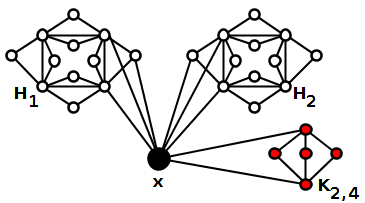
\includegraphics[width=5cm, center]{./img/grafoDobraExtremidadeObstruida2.png} &  &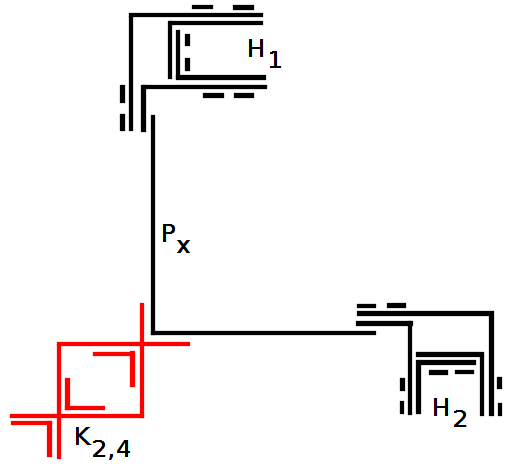
\includegraphics[width=6cm, center]{./img/extremidadeDobraObstruida5.png}  \\%[\abovecaptionskip]
    \footnotesize \centering (a) O grafo $G'$& & \footnotesize \centering (b)Uma representação $B_1$-EPG de $G'$%\\
 %   &&
  \end{tabular}
 \caption{Um exemplo de extremidade e dobra obstruída.} \label{fig:extremidadeDobraObstruida}
\end{figure}